\documentclass[fr]{../../../../../../eplexam}

\hypertitle{Théorie des graphes}{5}{INMA}{1961}{2016}{Janvier}{Mineure}
{Etudiants MAP de 2017}
{Vincent Blondel et Jean-Charles Delvenne}

\section{}
\begin{enumerate}
	\item Noé désire traverser la rivière avec son loup, sa chèvre et son chou. Seulement, il ne peut prendre qu’un seul de ces éléments avec lui dans sa barque, et il ne peut pas laisser le loup et la chèvre, ou la chèvre et le chou, seuls sans surveillance sur une des rives. Quel est le nombre minimum de traversées que Noé doit entreprendre pour rapatrier tout le monde sain et sauf d’une rive à l’autre ?

	\item On généralise à présent à un nombre quelconque d’être vivants dont certains ont des relations antagonistes. On peut modéliser la chaîne alimentaire par un graphe non-dirigé, où les noeuds sont les êtres vivants et une arête relie $u$ à $v$ si et seulement si $u$ mange $v$ ou $v$ mange $u$.  Pour un graphe quelconque, on va chercher la taille minimale de la barque pour que le problème soit soluble. Par taille, on entend le nombre d’êtres vivants qu’on peut embarquer en sus de Noé.
	Soit $S$ une couverture de sommets minimale du graphe. Démontrez que la taille minimale nécessaire de la barque est au moins $|S|$.
	
	\item Démontrez que la taille minimale nécessaire de la barque est au plus de $|S| + 1$.

	\item  Donnez un exemple de graphe pour lequel la taille minimale nécessaire de la barque est $|S|+1$.
	
	\begin{figure}[h!]
		\centering
		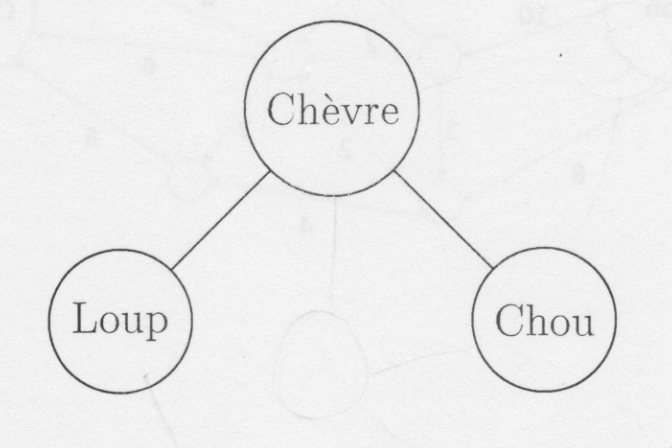
\includegraphics[scale=0.3]{fig1.PNG}
	\end{figure}

\end{enumerate}

\begin{solution}
	
\begin{enumerate}
	\item Au premier aller, il prendra la chèvre et la déposera de l'autre côté. Au deuxième aller, il prendra le loup et le déposera en reprenant la chèvre sur son retour et la déposant au point de départ. Il prend maintenant le chou et le dépose avec le loup de l'autre côté de la rive pour enfin prendre la chèvre et la déposer du bon côté. Il devra traverser 7 fois la rive.
	
	\item Au départ, tous les animaux sont d'un côté de la rive. A son premier allé, il est obligé de ne pas avoir de conflit entre les animaux restant au point de départ. Il laissera donc un set indépendant (animaux qui n'ont pas de conflit: qui ne sont pas adjacents). Donc, au premier trajet il y aura au moins une couverture de nos sommets dans la barque. Il faut donc minimiser la taille de la barque et donc prendre la couverture minimale. 
	
	\item 
	Propositions peu rigoureuses car elles ne \textit{démontrent} pas:
	\paragraph{Proposition 1}
	On prend la couverture minimale au premier trajet et donc ce qui reste sur la rive ne pose pas de problème. Puis à chaque voyage  suivant, on prend un animal en plus de la gauche vers la droite.
	\paragraph{Proposition 2}
	On met toute la couverture dans la barque et on la laisse jusqu'au dernier trajet. A chaque trajet, on prend un animal (c'est possible car il reste une place sur la barque). On peut donc amener les animaux un à la fois et terminer par déposer la couverture.
	
	\item  $|S| = 1$ mais insoluble si on ne peut prendre qu'un animal à la fois. Soit on commence par un autre que A et donc A mange les autres. Soit on commence par A mais au moment d'amener un deuxième, on doit le laisser avec A pour chercher un troisième et donc A le mange.
	
	\begin{solfig}{c}{Question 1.4}
		\centering
		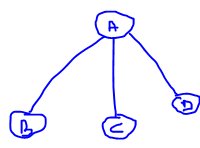
\includegraphics[scale=0.75]{jan2016Q1.PNG}
	\end{solfig}

\end{enumerate}	
	
\end{solution}

\section{}

On considère le problème du voyageur de commerce sur un graphe complet non-dirigé G, avec une distance $d_{uv}$ finie pour chaque paire de villes, et $d_{uu} = 0,\quad  \forall u$. On recherche donc le cycle hamiltonien le plus court. Par ailleurs, pour une ville $u$ quelconque on appelle un u\_arbre, un arbre sous-tendant les villes différentes de $u$, augmenté de deux arêtes incidentes à $u$.
\begin{enumerate}
	\item Démontrez que pour tout $u$, le u\_arbre de poids minimum a un poids inférieur ou  égal à la longueur du cycle hamiltonien le plus court.
	
	\item Proposez un algorithme efficace pour trouver le u-arbre de poids minimum, et analysez brièvement sa complexité.
	
	\item On considère la matrice symétrique des distances entre cinq villes :
	$$\begin{pmatrix}
	- & 40 & 40 & 30 & 60\\
	- & - & 60 & 40 & 50\\
	- & - & - & 40 & 30\\
	- & - & - & - & 50\\
	- & - & - & - & -\\
	\end{pmatrix}$$
	Votre patron est persuadé qu’il est possible de trouver un cycle hamiltonien de longueur totale de 170 kilomètres. Démontrez son erreur.
\end{enumerate}

\begin{solution}
	
	\begin{enumerate}
		
		\item On prend à la base le cycle hamiltonien le plus court. Par définition, il passe d'office par tous les sommets $u$. Pour chaque noeud, le cycle hamiltonien est un u\_arbre (le cycle hamiltonien moins le noeud $u$ est bien un arbre sous-tendant tous les noeuds sauf $u$. On ajoute les deux arêtes vers $u$ et on a bien un cycle hamiltonien.). Donc pour trouver le u\_arbre minimum pour un noeud $u$, la borne maximum est le cycle hamiltonien de base. On peut donc soit ne rien faire du tout soit uniquement faire mieux. Du coup, poids(u\_arbre minimum) $\leq$ longueur cycle hamiltonien minimum.
		
		\item On construit l'arbre sous-tendant de tous les noeuds excepté $u$ avec Kruskal et on rajoute les deux arêtes de poids minimum partant de $u$ vers les autres noeuds (?) 
		
		\item Raisonnement erroné du patron:
		
		\paragraph{Proposition 1}
		En représentant le graphe avec chaque arête ayant comme poids la distance entre les deux villes, et en cherchant le cycle hamiltonien de longueur minimum, on trouve une longueur totale de 190. 
		Alternativement, on construit un u\_arbre de longueur $>$ 170.
		\paragraph{Proposition 2}
		 On constate que pour faire un graphe hamiltonien de poids minimum, il faut d'office passer par 5 arêtes différentes. Les 5 arêtes les moins \textit{lourdes} dans ce cas-ci font respectivement $30-30-40-40-40$. Leur somme fait 180. En d'autres mots, même si on arrivait à faire un cycle hamiltonien avec ces 5 arêtes (ce qui serait alors d'office le cycle hamiltonien de poids minimum), la longueur serait de 180, ce qui est plus que 170.
		
	\end{enumerate}
	
\end{solution}

\section{}
\begin{enumerate}
	\item C’est l’été! Les Arlonnais se rendent en masse à Ostende pour profiter du soleil. Voici le réseau routier belge et la capacité de chacune de ses autoroutes en centaines de véhicules par heure. Quelle est la capacité totale du réseau routier entre Arlon et Ostende ? Expliquez votre démarche.
	
	\begin{figure}[h!]
		\centering
		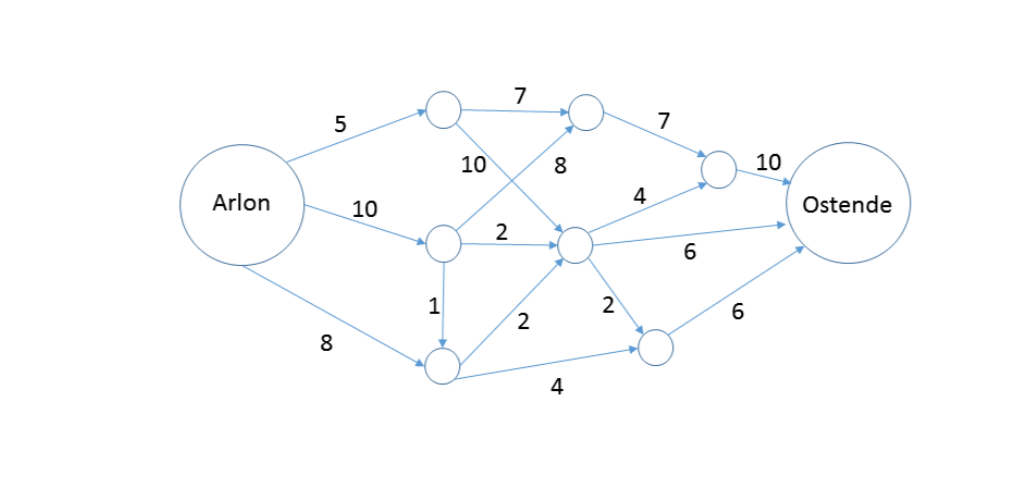
\includegraphics[scale=0.75]{flot.png}
		\caption{Flot}
	\end{figure}

	\item Les Décoréens du Nord veulent essayer leur nouvelle bombe N (qui crée des nids de poule capables de bloquer la circulation sur une route) en empêchant autant que possible les Arlonnais (dont la joie de vivre leur est insupportable) de se prélasser sur la plage. Quelle (unique) autoroute cibler pour réduire au maximum la capacité entre Arlon et Ostende ?
\end{enumerate}

\begin{solution}
	
	\begin{enumerate}
		
		\item Application de l'algorithme de Ford-Fulkerson, on trouve une capacité totale à Ostende de 20.
		
		\item Il faut cibler l'autoroute ayant un poids de 10 qui part de Arlon. 
		On trouve donc un flot maximal de 11 (l'arête de 5, l'arête de 2 ainsi que l'arête de 4 car le noeud aboutissant de l'autoroute supprimée est également supprimé) car nous savons que $$\mathrm{Flot}_{max}=\mathrm{Coupe}_{min}$$
		
	\end{enumerate}
	
\end{solution}

\section{}
 Vrai ou faux et justifiez:
\begin{enumerate}
	\item Deux représentations planaires d’un même graphe ont toujours le même nombre de faces.
	
	\item Tout graphe hamiltonien est 2-connexe.
	
	\item Tout graphe planaire possède un coloriage des noeuds à trois couleurs, tel que deux noeuds adjacents sont toujours de couleurs différentes.
	\item Tout arbre a un nombre chromatique de trois ou moins.
	
	\item Le polynôme chromatique de tout graphe qui possède une clique à sept noeuds a au moins cinq racines réelles.
\end{enumerate}

\begin{solution}
	
	\begin{enumerate}
		
		\item L'équation d'Euler nous dit qu'un graphe planaire respecte ceci: $n+f=2+e$. Si le graphe est le même, alors nous avons le même nombre d'arêtes ainsi que même nombre de noeuds. Nous avons donc bien pour chaque représentation $f=2+e-n$.
		
		\item Pour rappel, un graphe est dit $k$-connexe si enlever $k-1$ noeuds quelconques laisse le graphe connexe. Ici, $k=2$. La condition nécessaire pour qu'un graphe soit hamiltonien est que si on enlève $k$ noeuds quelconques d'un graphe, on obtient au plus $k$ composantes connexe.
		
		Un graphe hamiltonien possède un cycle hamiltonien ce qui implique que tous les noeuds sont reliés dans un cycle. Enlever n'importe quel noeud d'un cycle garde la connexité du cycle. Les graphes Hamiltoniens sont donc 2-connexe.
		
		\item Le graphe $K_4$ est planaire et son nombre chromatique est 4. Le graphe \textit{roue} avec un nombre pair de sommet est planaire mais son nombre chromatique est 4.
		
		\item 
		
		\item VRAI. S'il existe une clique à 7 noeuds dans le graphe, le nombre chromatique du graphe est au moins de 7. Le polynôme chromatique est défini comme le polynôme dont les racines sont les entiers positifs inférieurs au nombre chromatique. Dans notre cas, il y a au moins 0, 1, 2, 3, 4, 5 et 6, ce qui fait 7 racines réelles.
		
		On peut aussi se souvenir que le polynôme chromatique du graphe complet à $n = 7 $ noeuds est $P_n = \frac{t!}{(t-n)!}$.
		 
	\end{enumerate}
	
\end{solution}

\end{document}
